\documentclass{article}
\usepackage{graphicx} % Required for inserting images
\usepackage{appendix}
\usepackage{algorithm}
\usepackage{amssymb}
\usepackage{algpseudocode}
\usepackage{amsmath}
\usepackage{biblatex}
\addbibresource{references.bib}

% Set vertical spacing within sections
\newlength{\sectionvspace}
\setlength{\sectionvspace}{1em}



\title{AI-Enhanced Fast Cosmological Simulations for Accurate Large-Scale Structure Inference}
\author{David Amrein }
\date{\today}

\begin{document}

\maketitle

\tableofcontents

\newpage
\begin{abstract}
    
\end{abstract}

\section{Introduction}
\section{Theoretical Background}

\subsection{Cosmological Framework}

\subsubsection{The Cosmic Web}
\label{sec:cosmic_web}

On scales of a few to a few hundred megaparsecs, matter in the Universe is not smoothly distributed but arranged into an interconnected network of dense compact knots, elongated filaments, two-dimensional sheets, and large under-dense voids -- collectively known as the \emph{cosmic web} \cite{bond_how_1996, libeskind_tracing_2018}. The term originates with \citeauthor{bond_how_1996}, who showed that this filament-dominated pattern is already present in embryonic form in the tidal field of the initial density perturbations, with the nonlinear gravitational evolution sharpening rather than creating it \cite{bond_how_1996}. The same gravitational instability that seeds this pattern is responsible for its growth: initially small density fluctuations are amplified by their own self-gravity, so that overdense regions contract while voids expand and come to dominate the volume of the Universe \cite{bond_how_1996}. Large galaxy redshift surveys -- 2dFGRS, SDSS, and the 2MASS redshift survey (2MRS) among them -- as well as cosmological $N$-body simulations both recover this same web-like arrangement of galaxies and dark matter \cite{libeskind_tracing_2018}.
\vspace{\sectionvspace} \\ 
Gravitational instability drives the emergence of anisotropic structure: because collapse along the direction of a region's strongest tidal compression proceeds fastest, an initially only mildly non-spherical overdensity first flattens into a sheet, then contracts further into a filament, and only finally collapses fully into a compact halo -- the sequence of anisotropic collapse first described by Zel'dovich \cite{libeskind_tracing_2018}. This picture can be made quantitative by looking at the local tidal (or velocity-shear) field. Following the tidal-tensor classification reviewed by \cite{libeskind_tracing_2018}, one computes the Hessian of the (rescaled) gravitational potential $\phi$,
\begin{equation}
  T_{\alpha\beta} = \frac{\partial^2 \phi}{\partial x_\alpha \partial x_\beta}, \qquad \nabla^2 \phi = \delta,
  \label{eq:tidal_tensor}
\end{equation}
where $\delta = (\rho - \bar\rho)/\bar\rho$ is the dimensionless matter overdensity and $\phi$ has been normalised by $4\pi G \bar\rho$ so that Eq.~\eqref{eq:tidal_tensor} takes the form of the Poisson equation \cite{libeskind_tracing_2018}. Diagonalising the (real, symmetric) tidal tensor at each point gives three eigenvalues $\lambda_1 > \lambda_2 > \lambda_3$; counting how many of them exceed a chosen threshold $\lambda_{\rm th}$ classifies that point as part of a void (zero eigenvalues above threshold), a sheet (one), a filament (two), or a knot (three) \cite{libeskind_tracing_2018}. Voids, sheets, filaments and knots are thus not four independent morphologies but a nested hierarchy, each embedded within the next.

\subsubsection{Matter Power Spectrum and Transfer Function}
\label{sec:power_spectrum}

While the tidal-tensor classification above describes the cosmic web \emph{qualitatively}, its statistical properties are quantified through the matter power spectrum $P(k)$. Writing the density contrast in Fourier space as $\delta(\mathbf{k})$, and assuming statistical homogeneity and isotropy, the power spectrum is defined through
\begin{equation}
  \big\langle \delta(\mathbf{k})\, \delta^*(\mathbf{k}')\big\rangle = (2\pi)^3\, \delta_D(\mathbf{k}-\mathbf{k}')\, P(k),
  \label{eq:power_spectrum_def}
\end{equation}
where $\delta_D$ is the Dirac delta and the angle brackets denote an ensemble average over realisations of the initial conditions. \cite{dodelson_modern_2020, huterer_growth_2023} Simplified we can express it
\begin{equation}
    P(k) \propto k^{n_s}T^2(k)
\end{equation}
with $n_s$ the scalar spectral index. \cite{huterer_growth_2023, eisenstein_baryonic_1998} Further we can simplify the transfer function $T(k)$ to 
\begin{equation}
    T(k) = 1 - \frac{k}{k_{eq}} + ...  
\end{equation}
with $k_{eq} = H_0\sqrt{\frac{2\Omega_m}{\Omega_r}}$. \cite{bardeen_statistics_1986, eisenstein_baryonic_1998} We see that the transfer function is an essential component of the power matter spectrum, as also the matter and radiation density. We also see that transfer function is dependent on the neutrino mass, as visualized in Figure \ref{fig:transfer_function}. 
\begin{figure}[h!]
    \centering
    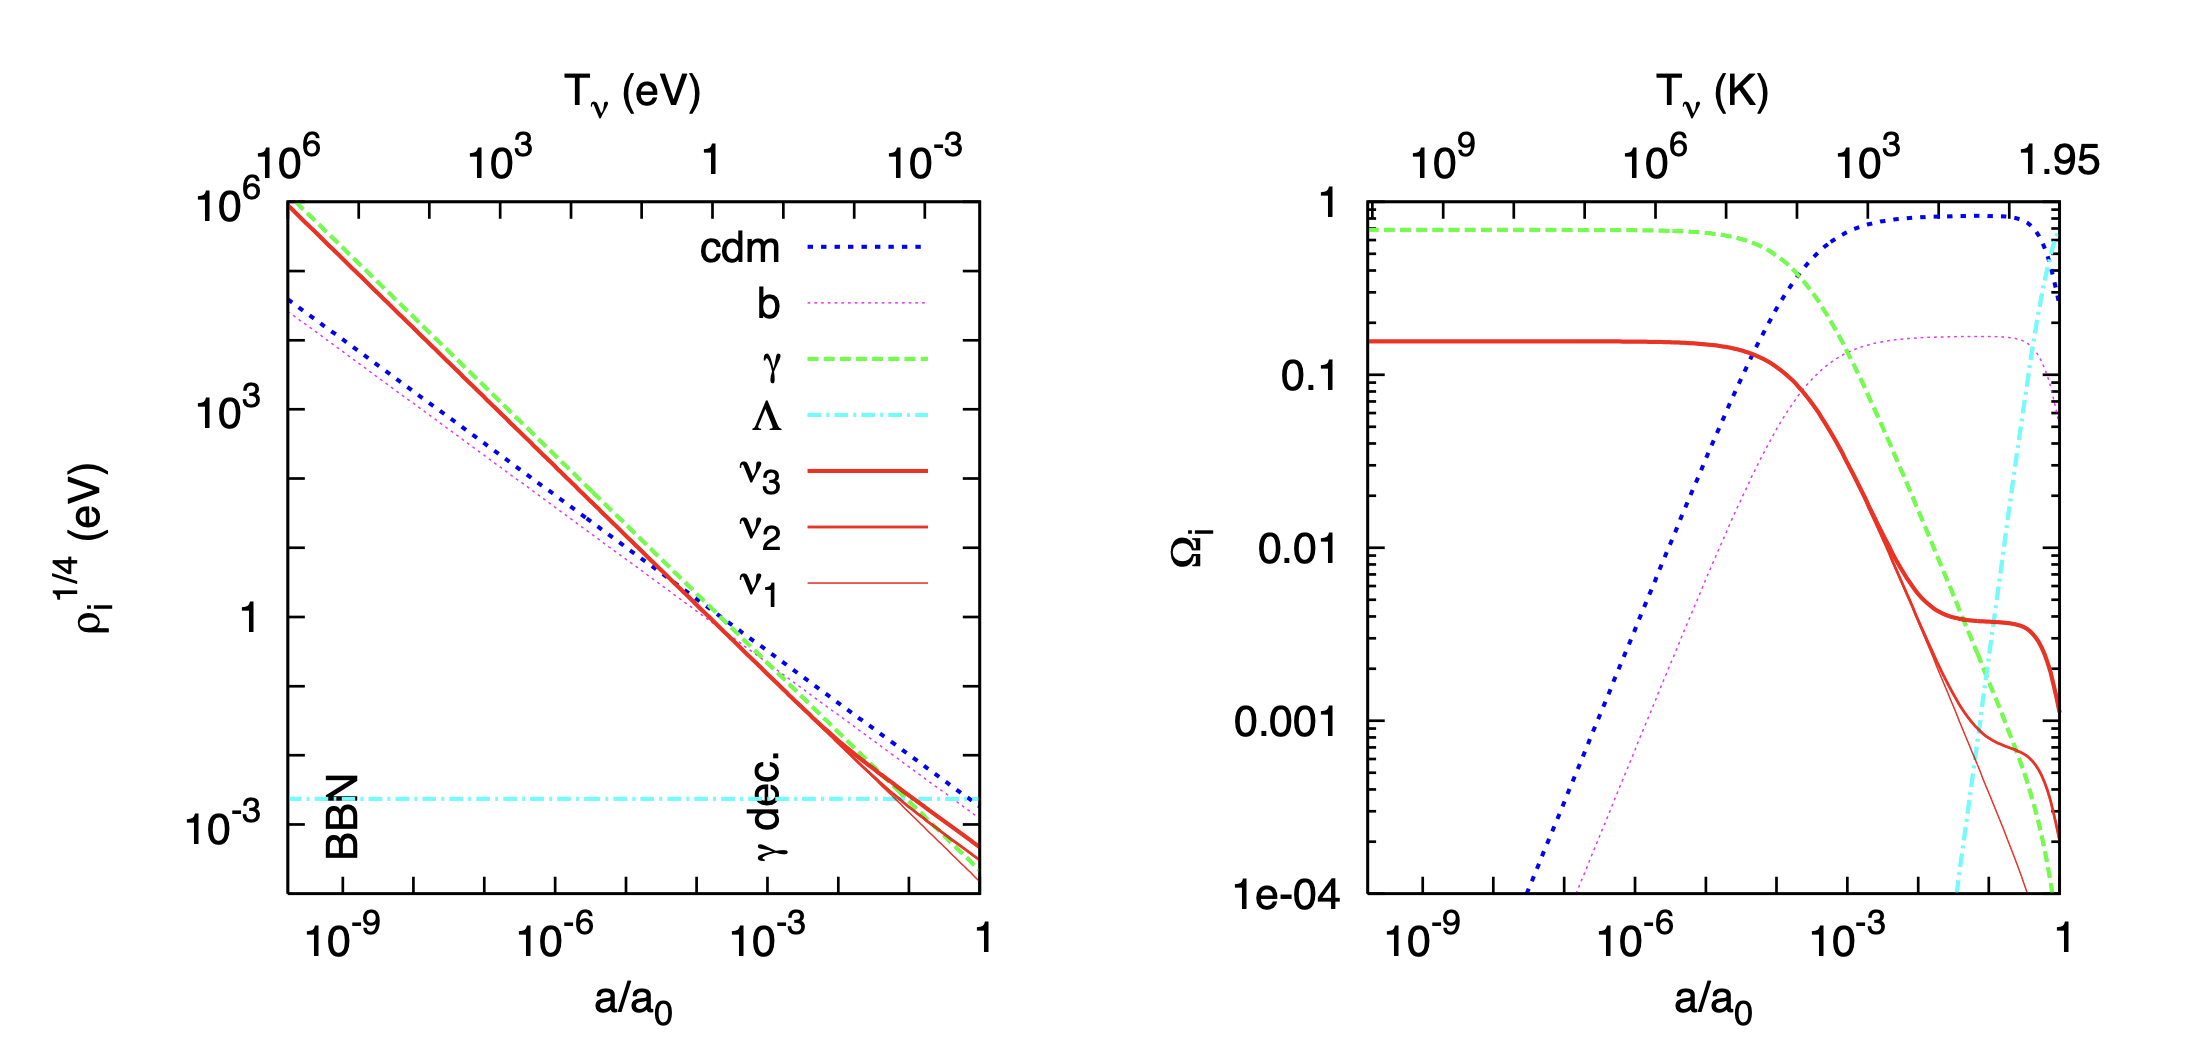
\includegraphics[width=0.8\linewidth]{plots/background/transfer_function.png}
    \caption{\cite{lesgourgues_massive_2006}}
    \label{fig:transfer_function}
\end{figure}
There are three red curves regarding the neutrino mass $m_{\nu_1}=0$, $m_{\nu_2} = 0.009$ and $m_{\nu_3} = 0.05$ eV. \cite{lesgourgues_neutrino_2012,lesgourgues_massive_2006} Also this will have a an effect on angular power spectrum $C_l$, which is defined as
\begin{equation}
    C_l \approx \int  k^2P(k) dk
\end{equation}
is the fourier transfrom of the power matter spectrum. \cite{seljak_line_1996}.
\begin{figure}
    \centering
    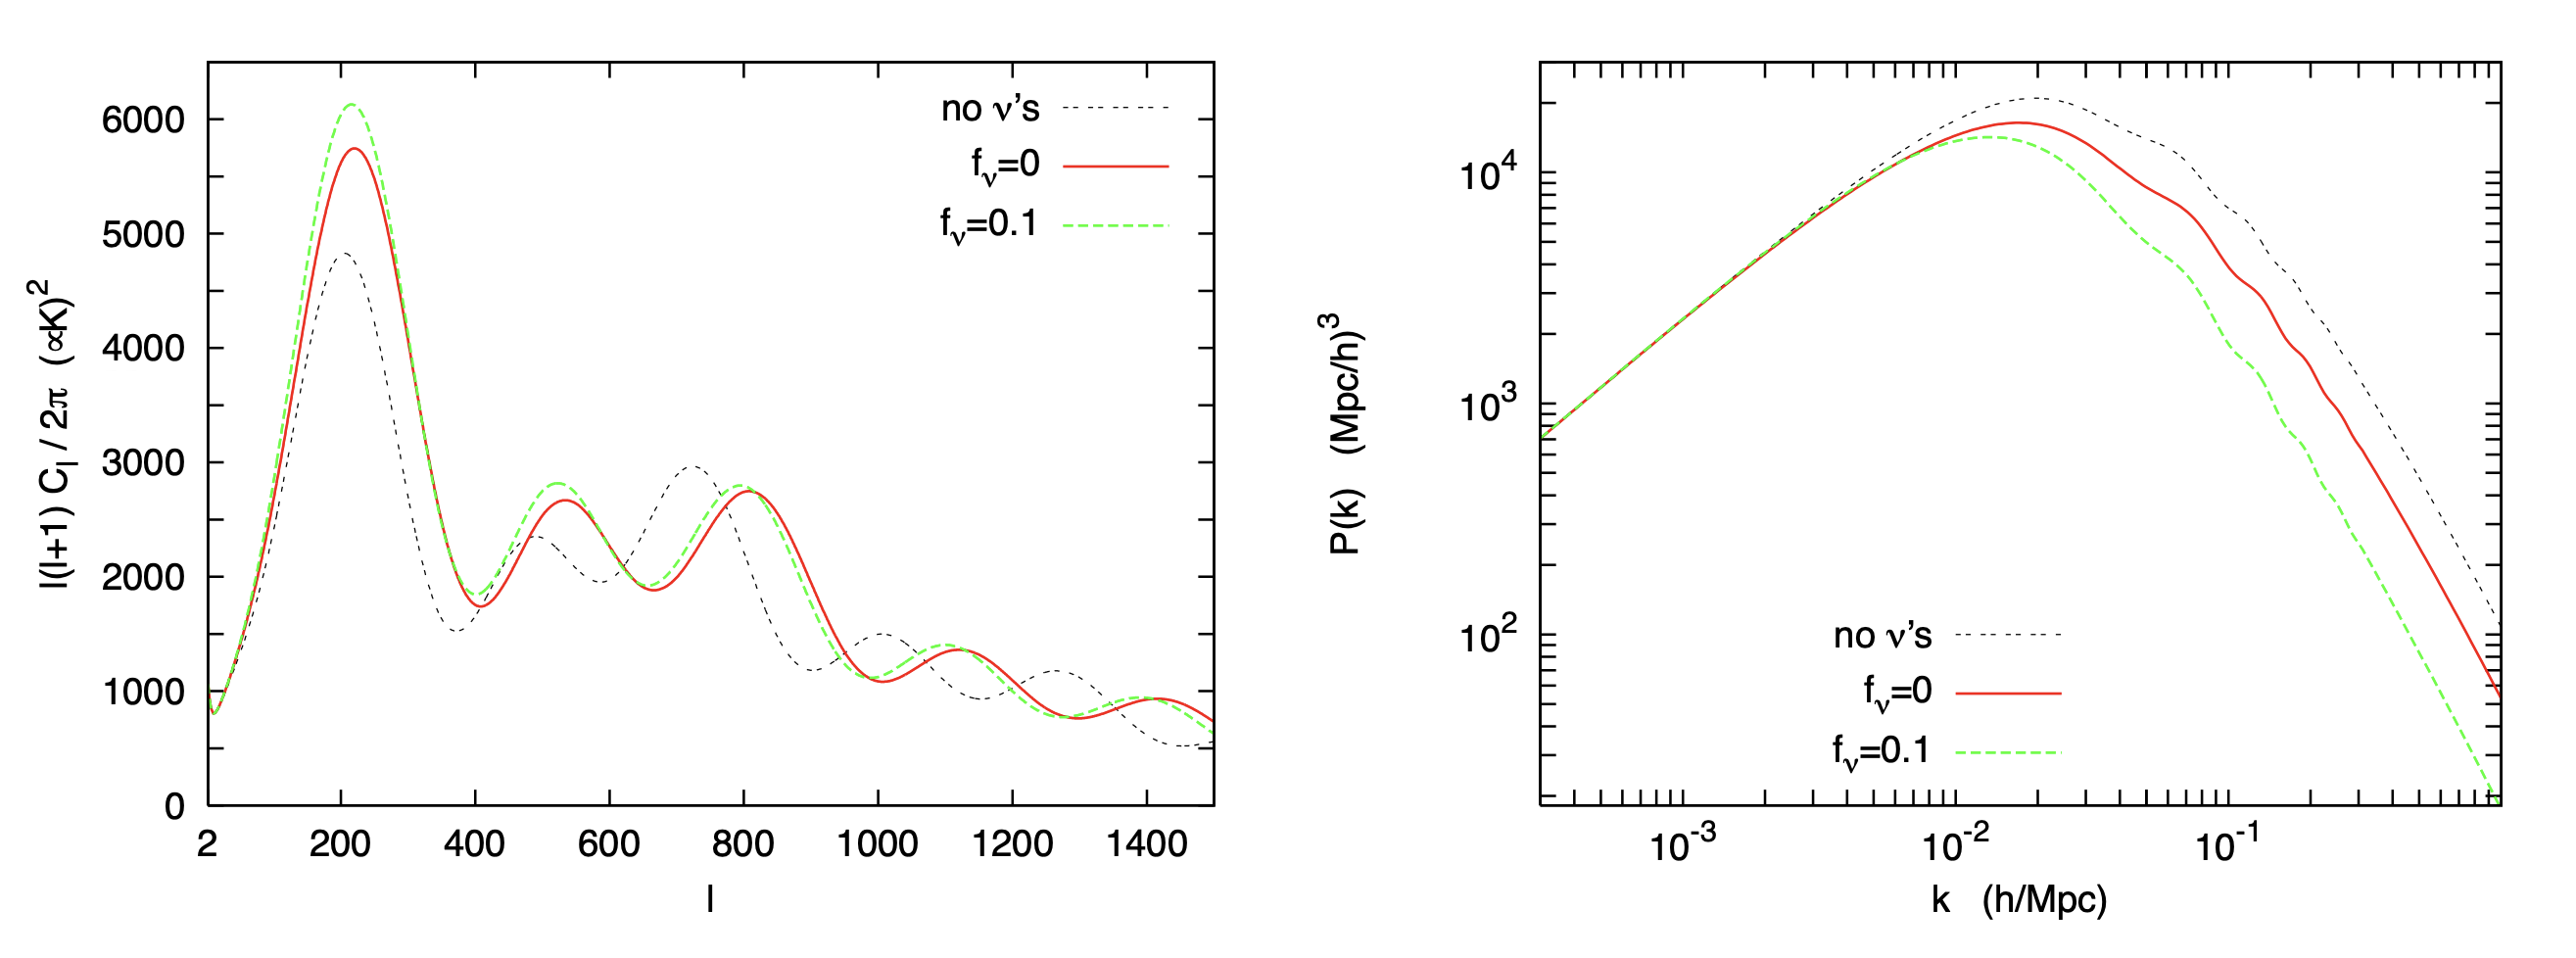
\includegraphics[width=0.8\linewidth]{plots/background/neutrinos_effect.png}
    \caption{\cite{lesgourgues_massive_2006}}
    \label{fig:placeholder}
\end{figure}
This fundamental for this project since later we will see its influence, when generating the initial conditions for the simulations. 
\vspace{\sectionvspace} \\
Obtaining $P(k)$ precisely, including this transfer function, requires solving the coupled linear Einstein--Boltzmann equations for the perturbed Friedmann--Lema\^itre--Robertson--Walker metric and the phase-space distributions of all matter and radiation species -- the same system solved by the differentiable Einstein--Boltzmann module of the Disco-DJ framework used later in this thesis \cite{hahn_disco-dj_2024}.

\subsubsection{Lightcones and Snapshots}

An $N$-body simulation naturally outputs \emph{snapshots}: the full particle phase-space (positions and velocities) within a periodic box of fixed comoving side length, at a fixed time. Reproducing how we actually observe the Universe, however, requires a \emph{lightcone}: rather than a single time slice, an observer at a fixed spacetime point receives light emitted from progressively more distant (and hence earlier) shells as one looks to higher redshift, so a simulated lightcone must record particles at the (redshift-dependent) comoving distance from which they are being observed, not at a single global time.
\vspace{\sectionvspace} \\
Because the depth of the desired lightcone (out to some $z_{\max}$) is typically larger than a single simulation box, the box is periodically replicated around a centrally placed observer: box replication takes advantage of the fact that a simulation with periodic boundary conditions can, in principle, represent an arbitrarily large volume, at the cost of the same structures reappearing at multiple replica images along a given line of sight \cite{kacprzak_cosmogridv1_2023}. This replication strategy, and the trade-off between box size, structure repetition, and the resulting bias or excess variance in the projected lightcone statistics, is discussed in detail by \cite{kacprzak_cosmogridv1_2023}, who additionally introduce a shell-permutation scheme that mitigates the repeated-structure problem by drawing different radial shells of a single lightcone from independent simulations of the same cosmology.

\subsection{Cosmological Simulations}

Cosmological $N$-body simulations have historically tracked, and in some respects driven, the development of high-performance computing: the number of particles that can be evolved in a fixed wall-clock time has grown by many orders of magnitude over the past decades, both because of raw hardware improvements and because of continual gains in the efficiency of the gravity solvers themselves \cite{potter_pkdgrav3_2016}. The scientific payoff of these simulations lies in their ability to model the large-scale structure (LSS) of the Universe to the non-linear precision that photometric surveys require. LSS observables are particularly sensitive to the present-day matter density $\Omega_m$ and the amplitude of matter clustering $\sigma_8$; because a lightcone simulation can be sliced into tomographic redshift bins, it further allows the growth of structure to be tracked over cosmic time, which is what makes such simulations sensitive to the dark-energy equation-of-state parameter $w_0$ (and its possible time evolution) and hence to the physical origin of cosmic acceleration \cite{kacprzak_cosmogridv1_2023}.

\subsubsection{DISCO-DJ}

All forward models implemented in Disco-Dj are concerned with computing an approximate solution to the cosmological Vlasov–Poisson system: 

df dt = ∂tf + p  a2 · ∇xf + g  a · ∇pf = 0, where g := −∇xφ, (2.1)  see e.g. [56, 57] for recent reviews. Here, f = f (x, p, t) is the phase-space distribution function, where the coordinates x are comoving in a universe expanding with a scale factor a(t).

We now turn towards the ingredients for PM (particle mesh) simulations. A key component is the time integration scheme used for the temporal discretisation of the Vlasov–Poisson system (2.1). To make a connection with the previous sections, we note that it is possible in fact to design integrators that exactly trace perturbative trajectories up to a certain order, while higher-order truncation errors decrease as the step size is reduced [78–80]. A single PM time step would then compute, e.g., 2LPT trajectories (up to higher-order terms, and with the caveat that discretisation errors arise due to the Eulerian PM-based force computation, compared to the Lagrangian evaluation of quantities in LPT).  Disco-Dj supports different drift-kick-drift leapfrog/Verlet steppers of the form: 

X n+1/2  i = Xn  i + τ1V n  i ,  V n+1  i = αV n  i + βA(Xn+1/2  i ),  X n+1  i = X n+1/2  i + τ2V n+1  i .
Here, Xn  i denotes the position of particle i at the nth time step, A(Xn+1/2  i ) is the acceleration evaluated in the middle of the full time step (i.e. after the first drift), τ = τ1 + τ2 is the time step size, and α and β are coefficients that may depend on both the current time and time step. For the velocity variable V n  i (and the associated time step variable τ ), different choices are supported, such as  • the canonical momentum variable V = a2X ̇ with τ = R an+1  an (H(a)a3)−1 da and  • the growth-time velocity V = dX/dD = X ̇ /(aH(a)D′(a)) with τ = Dn+1 − Dn,  where the overdot denotes a derivative w.r.t. cosmic time. symplectic Zeldovich consistent integrator.  Recently, Ref. [80] built onto the analysis of Ref. [79] and derived the BullFrog integrator, which corresponds to the unique choice of α and β that aligns the N -body trajectory with 2LPT after each time step in its regime of validity:  α = E′(Dn+1) − ξn+1/2  E′(Dn) − ξn+1/2  , β = (1 − α)Dn+1/2, (2.16)  – 10 where  ξ = D−1  n+1/2 En + E′(Dn) Dn+1 − Dn  2 − Dn+1/2, (2.17)  and E = −(3/7)D2 − (3/1001)ΛD5 + O(Λ2D8) with Λ := ΩΛ/Ωm is the second-order growth function (see Appendix B for the defining ordinary differential equation). 1 In view of its superior performance, BullFrog is the default integrator in DiscoDJ, yielding accurate predictions already with very few steps. \cite{list_disco-dj_2026}

\subsubsection{Pkdgrav}

The gravity solver \textsc{PkdGrav3} computes the gravitational force with a binary-tree Fast Multipole Method (FMM): rather than only approximating a distant tree cell's effect on individual particles (as in a Barnes--Hut tree code), it also expands the potential \emph{within} a receiving cell sourced by a distant cell, an interaction that lets the cost of a full force evaluation scale as $\mathcal{O}(N)$ instead of $\mathcal{O}(N\log N)$ \cite[Sec.~3.1]{potter_pkdgrav3_2016}. \vspace{\sectionvspace} \\ 
Because particles in different regions of a cosmological box span many orders of magnitude in local density, and hence in dynamical time, a single global time step would be highly wasteful. \textsc{PkdGrav3} instead assigns each particle to one of several time-step ``rungs'', advancing only the particles active on a given rung at each sub-step, and additionally builds a second, smaller tree restricted to the small subset of particles on the shortest (``very active'') rungs so that this frequently-rebuilt tree stays cheap; the combination is summarised by the kick-drift-kick ``umbrella'' diagram over one base time step, see Figure \ref{fig:pkd_rungs}. This dual-tree multi-stepping scheme is what keeps the tree-construction cost from dominating the runtime even though the shortest rungs may be walked hundreds of times per base step \cite[Sec.~3.2]{potter_pkdgrav3_2016}. \vspace{\sectionvspace} \\ 

\begin{figure}[h!]
    \centering
    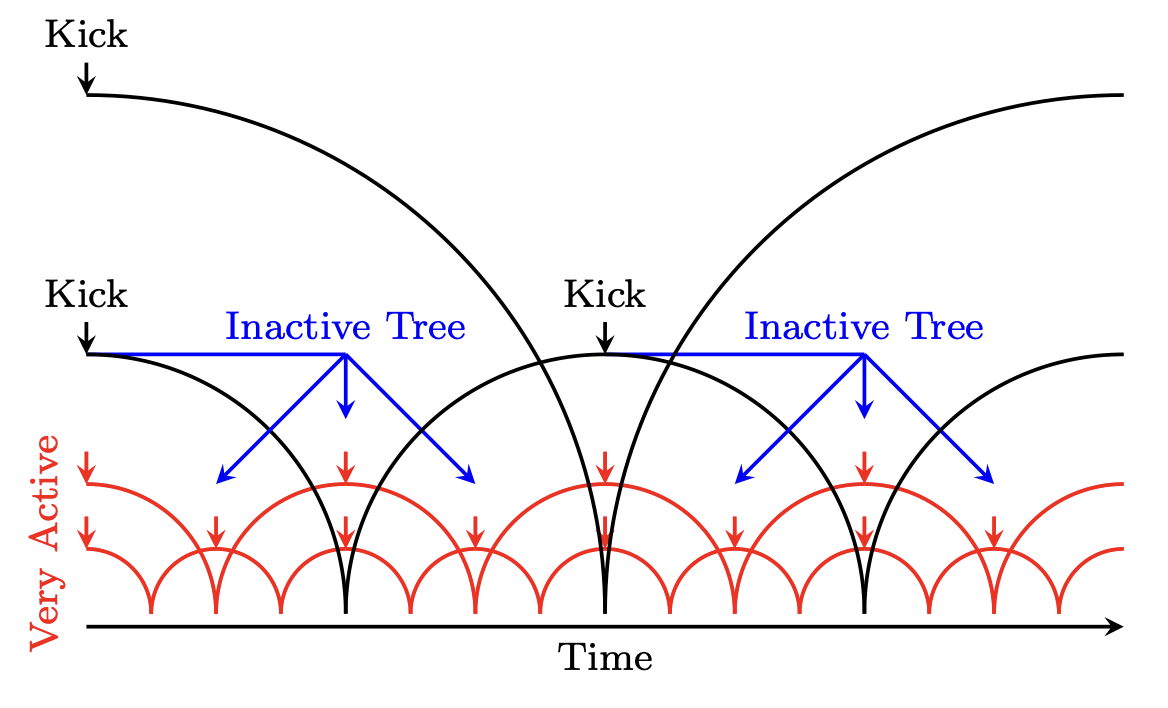
\includegraphics[width=0.5\linewidth]{plots/background/pkdgrav_rungs.png}
    \caption{\cite{potter_pkdgrav3_2016}}
    \label{fig:pkd_rungs}
\end{figure}

\subsubsection{CosmoGridV1}

CosmoGridV1 is a large, publicly released suite of lightcone $N$-body simulations built specifically for map-level (rather than two-point-function-only) cosmological inference from large-scale-structure probes such as weak lensing and galaxy clustering \cite{kacprzak_cosmogridv1_2023}. It samples a six-dimensional flat $w$CDM parameter space ($\Omega_m$, $\sigma_8$, $w_0$, $H_0$, $n_s$, $\Omega_b$, with a fixed total neutrino mass) at 2500 points arranged on a Sobol sequence, running 7 independent realisations at every point, in addition to 200 realisations (with parameter-derivative pairs) at a fixed fiducial cosmology and a smaller set of benchmark runs at higher resolution used to validate the main configuration's choices of box size, particle count, and shell thickness \cite{kacprzak_cosmogridv1_2023}. Every simulation is run with \textsc{PkdGrav3} in a periodic box of $900\,\mathrm{Mpc}/h$ with $832^3$ particles, and stores its lightcone as HEALPix particle-count maps at $N_{\rm side}=2048$ out to $z=3.5$, together with friends-of-friends halo catalogues at each output step \cite{kacprzak_cosmogridv1_2023}. These raw particle-count shells are the basis from which observable maps of weak-lensing convergence, galaxy clustering, and intrinsic alignment are subsequently constructed, and the same dataset has previously been used, together with a shell-based baryon correction model, for a deep-learning cosmological parameter analysis of the KiDS-1000 weak-lensing survey \cite{fluri_full_2022}.


\section{Methods and implementation}
\subsection{Pipeline Architecture}
\underline{Limitations and Solutions}

The problem of comosgrid an pkdgrav is that we have much longer simulation time.
The alternative framework to it is by using the fast disco simulation. The tradeoff we have with disco here is that we have less precision on small scales. So to overall goal is:

Let $f(Map)$ be some small scale corrections function

\[
f(Map_{disco}) \approx Map_{Cosmogrid}
\]


First we planned to do an AI-correction, but a better approach was with correcting the angular power matter spectrum for high dipole l.  


\subsection{IC generation}
\label{sec:ic_generation}

\subsubsection{Validation against CosmoGridV1}

Before using \textsc{disco}'s shell builder (Sec.~\ref{sec:shell_builder_core}) for any downstream analysis, we first validate that a lightcone produced with our \textsc{PkdGrav3} configuration reproduces the reference CosmoGridV1 statistics. To this end we run \textsc{PkdGrav3} with its native lightcone module on the exact box, resolution, and cosmology used by CosmoGridV1, and compare the resulting matter angular power spectrum $C_\ell$ against the corresponding CosmoGridV1 lightcone. Table~\ref{tab:pkdgrav_params} lists the parameters that must be matched exactly for this comparison to be meaningful, together with the corresponding keys in the \textsc{PkdGrav3} configuration file (\texttt{cosmology.par}).

\subsubsection{Backscaled initial conditions and hand-off to \textsc{disco}}

As described in section \ref{sec:power_spectrum} we have to ensure that we are dealing with deliver a correct transfer function with the correct neutrino mass. Since this has an influence on directly, if it matches the cosmogridv1. 

The resulting particle positions and velocities at $a_i = 1/(1+z_i)$ are exported and used, unmodified, as the initial condition for the corresponding \textsc{disco} run: \textsc{disco} evolves this state forward to $a=1$ and accumulates the lightcone with the shell builder of Sec.~\ref{sec:shell_builder_core} over the same redshift range, $z_{\max}=3.5$ down to $z=0$, at the same HEALPix resolution $N_{\mathrm{side}}=2048$.
\subsection{Shell Builder}

\subsubsection{Core}
\label{sec:shell_builder_core}

A lightcone output requires the particle distribution to be resampled at every integration step, since the observable past lightcone shell changes continuously as the universe evolves. The most direct implementation stores the full particle snapshot at each of the $n_{\mathrm{steps}}$ integration steps and performs the shell decomposition after the simulation has finished. This approach is memory-prohibitive: retaining $n_{\mathrm{steps}}$ full-resolution snapshots simultaneously exceeds the available device memory for the particle counts considered here. We therefore interleave the shell decomposition with the time integration, so that at any given time only the particle states immediately before and after the current integration step, together with a set of low-dimensional pixelized count maps, need to be held in memory.

\paragraph{Time discretization.}
The radial shells are not defined by the integrator itself but are supplied externally, e.g.\ through a CosmoGridV1-format metainfo table. Each shell $s \in \{1,\dots,S\}$ is specified by a redshift interval $[z_s^{\mathrm{lo}}, z_s^{\mathrm{hi}}]$ and the corresponding comoving-distance interval $[r_s^{\mathrm{lo}}, r_s^{\mathrm{hi}}]$. To ensure that no shell boundary is crossed \emph{within} an integration step, we define the set of integration times as the union of all shell edges,
\begin{equation}
  \{z_j\}_{j=0}^{S} = \mathrm{unique}\Big(\{z_s^{\mathrm{lo}}\}_{s=1}^{S} \,\cup\, \{z_s^{\mathrm{hi}}\}_{s=1}^{S}\Big), \qquad a_j = \frac{1}{1+z_j},
  \label{eq:step_grid}
\end{equation}
sorted in ascending order of $a_j$ (equivalently, descending order of $z_j$). By construction, every shell boundary coincides exactly with an integration-step boundary. The interval $[a_{\mathrm{ini}}, a_0]$, preceding the first shell, is integrated separately with $n_{\mathrm{pre}}$ sub-steps and without shell accumulation, in order to bring the particle state into registry with the shell grid defined in Eq.~\eqref{eq:step_grid}. The remaining $J = S$ intervals $[a_j, a_{j+1}]$, $j = 0,\dots,J-1$, are each advanced with exactly one integration sub-step.

\paragraph{Accumulation procedure.}
Algorithm~\ref{alg:shell_accum} summarizes the per-step accumulation. At step $j$, the comoving positions and validity mask of all particles are recorded both before the sub-step, $\{\mathbf{x}_p^{(j)}, m_p^{(j)}\}$, and after it, $\{\mathbf{x}_p^{(j+1)}, m_p^{(j+1)}\}$. The scale-factor edges of the step are converted to comoving distance through the cosmology-dependent map $\chi(a)$,
\begin{equation}
  R_j = \chi(a_j), \qquad R_{j+1} = \chi(a_{j+1}), \qquad R_j > R_{j+1},
  \label{eq:step_radii}
\end{equation}
where the inequality follows from $\chi$ being strictly decreasing on $a \in (0,1]$. The set of shells that are traversed during step $j$ is
\begin{equation}
  \mathcal{A}_j = \big\{\, s \;:\; r_s^{\mathrm{lo}} < R_j \ \wedge\ r_s^{\mathrm{hi}} > R_{j+1} \,\big\},
  \label{eq:active_shells}
\end{equation}
i.e.\ those shells whose radial bin overlaps the annulus $[R_{j+1}, R_j)$ swept out during the step. For each active shell $s \in \mathcal{A}_j$, the pre- and post-step particle states, together with the radial bounds $(r_s^{\mathrm{lo}}, r_s^{\mathrm{hi}})$, are passed to the shell-accumulation routine described in Sec.~\ref{sec:crossing}, which returns a HEALPix pixel count map $\mathbf{M}_s^{(j)} \in \mathbb{N}^{N_{\mathrm{pix}}}$. This map is added to a running total,
\begin{equation}
  \mathbf{S}_s \;\mathrel{+}=\; \mathbf{M}_s^{(j)}, \qquad s \in \mathcal{A}_j.
  \label{eq:shell_update}
\end{equation}
Because the integration grid is constructed from the shell edges themselves (Eq.~\ref{eq:step_grid}), $\mathcal{A}_j$ reduces to a single shell in the generic case; the overlap criterion in Eq.~\eqref{eq:active_shells} is retained in its general form to also cover degenerate or adjacent bins in the input shell table.

\begin{algorithm}[h!]
\caption{Streaming shell accumulation}
\label{alg:shell_accum}
\begin{algorithmic}[1]
\State Load shell table $\{(z_s^{\mathrm{lo}}, z_s^{\mathrm{hi}}, r_s^{\mathrm{lo}}, r_s^{\mathrm{hi}})\}_{s=1}^{S}$; build integration grid $\{a_j\}_{j=0}^{J}$ (Eq.~\ref{eq:step_grid})
\State Initialize $\mathbf{S}_s \gets \mathbf{0}$ for all $s$
\State Integrate particle state from $a_{\mathrm{ini}}$ to $a_0$ with $n_{\mathrm{pre}}$ sub-steps (no accumulation)
\For{$j = 0, \dots, J-1$}
  \State Record pre-step positions and mask, $\{\mathbf{x}_p^{(j)}, m_p^{(j)}\}$
  \State Integrate one sub-step: $a_j \rightarrow a_{j+1}$
  \State Record post-step positions and mask, $\{\mathbf{x}_p^{(j+1)}, m_p^{(j+1)}\}$
  \State Compute $R_j, R_{j+1}$ (Eq.~\ref{eq:step_radii}) and active shells $\mathcal{A}_j$ (Eq.~\ref{eq:active_shells})
  \For{$s \in \mathcal{A}_j$}
    \State $\mathbf{M}_s^{(j)} \gets$ crossing map from $\{\mathbf{x}_p^{(j)}, \mathbf{x}_p^{(j+1)}, m_p^{(j)}, m_p^{(j+1)}\}$ restricted to $[r_s^{\mathrm{lo}}, r_s^{\mathrm{hi}})$ (Sec.~\ref{sec:crossing})
    \State $\mathbf{S}_s \mathrel{+}= \mathbf{M}_s^{(j)}$
  \EndFor
  \State Discard pre-step state; retain post-step state as pre-step state for $j+1$
\EndFor
\State \Return $\{\mathbf{S}_s\}_{s=1}^{S}$
\end{algorithmic}
\end{algorithm}

\paragraph{Output.}
Once all $J$ steps have been processed, the set of per-shell count maps $\{\mathbf{S}_s\}_{s=1}^{S}$, together with the shell table, is serialized to a single output file. At no point during the procedure are more than $\mathcal{O}(1)$ full particle snapshots and $S$ integer-valued maps of size $N_{\mathrm{pix}}$ held simultaneously; this is what removes the memory bottleneck associated with the naive end-of-run decomposition.
\subsubsection{Crossing Condition}
\label{sec:crossing}

 The condition follows the moving-lightcone formulation of \textsc{PkDgrav3} \cite{noauthor_examplepkdgrav3_lightcone_2022} exactly, rather than the vector-trajectory intersection used in the earlier sketch.

\paragraph{Periodic replicas.}
The observer is placed at the box centre, $\mathbf{o} = (L/2, L/2, L/2)$, with $L$ the box side length. Since the requested lightcone depth $\chi_{\max} = \chi\big(1/(1+z_{\max})\big)$ generally exceeds $L$, the simulation volume is periodically replicated: let

\begin{equation}
  \mathcal{D} = \Big\{\, \mathbf{d} = (n_1, n_2, n_3)\,L \;:\; \mathbf{n}\in\mathbb{Z}^3, \ \; \text{replicated cube intersects the ball of radius } \chi_{\max} \text{ about } \mathbf{o} \,\Big\}
  \label{eq:replica_set}
\end{equation}

denote the finite set of replica offsets, precomputed once from $(\chi_{\max}, L)$. For each $\mathbf{d}\in\mathcal{D}$ we also precompute the nearest and farthest possible distance of the replicated cube from the observer,
\begin{equation}
  r_{\min}(\mathbf{d}) = \big\lVert \max(0, |\mathbf{d}| - L/2) \big\rVert, \qquad
  r_{\max}(\mathbf{d}) = \big\lVert |\mathbf{d}| + L/2 \big\rVert,
  \label{eq:replica_bounds}
\end{equation}
(componentwise $\max$ and absolute value, followed by the Euclidean norm), which allow a replica to be rejected for a given step without evaluating any particle if its radial range cannot overlap the step's lightcone annulus.

\paragraph{Linear crossing formula.}
For step $j$ with N-body boundaries $a_j < a_{j+1}$, define, as before, $r_j^{\mathrm{hi}} = \chi(a_j)$ and $r_j^{\mathrm{lo}} = \chi(a_{j+1})$. For a particle with pre-/post-step positions $\mathbf{x}_p(a_j), \mathbf{x}_p(a_{j+1})$ relative to the box centre, and a replica offset $\mathbf{d}\in\mathcal{D}$, define the shifted positions and their radii
\begin{equation}
  \mathbf{R}_0 = \mathbf{x}_p(a_j) + \mathbf{d}, \qquad \mathbf{R}_1 = \mathbf{x}_p(a_{j+1}) + \mathbf{d}, \qquad
  r_0 = \lVert \mathbf{R}_0 \rVert, \qquad r_1 = \lVert \mathbf{R}_1 \rVert.
  \label{eq:replica_radii}
\end{equation}
Rather than solving for the intersection of the interpolated \emph{vector} trajectory with the receding lightcone sphere (which requires a quadratic root), the implementation follows \textsc{PkDgrav3} and linearly interpolates the \emph{scalar} radii of the particle and of the lightcone front over the step,
\begin{equation}
  r_p(v) = r_0 + v\,(r_1 - r_0), \qquad R(v) = r_j^{\mathrm{hi}} - v\,(r_j^{\mathrm{hi}} - r_j^{\mathrm{lo}}), \qquad v\in[0,1],
  \label{eq:scalar_interp}
\end{equation}
and solves $r_p(v^\ast) = R(v^\ast)$ for the crossing parameter,
\begin{equation}
  v^\ast = \frac{r_j^{\mathrm{hi}} - r_0}{\big(r_j^{\mathrm{hi}} - r_j^{\mathrm{lo}}\big) + (r_1 - r_0)}.
  \label{eq:vx_formula}
\end{equation}
A particle--replica pair is accepted only if $v^\ast \in [0,1)$; since Eq.~\eqref{eq:vx_formula} partitions the step interval, this guarantees that every particle is caught in \emph{at most one} step, for a fixed replica -- evaluating the crossing test against the (generally narrower) metainfo shell bounds instead of the full step bounds $[r_j^{\mathrm{lo}}, r_j^{\mathrm{hi}})$ would break this partition and could double-count particles moving across two adjacent shells within the same step. Pairs with $|r_1 - r_0|$ below a numerical tolerance ($10^{-20}$) are treated as non-moving and rejected, and the denominator of Eq.~\eqref{eq:vx_formula} is floored in magnitude at $10^{-10}$ to avoid division by a near-zero value.

\paragraph{Shell assignment and pixelization.}
The crossing position is obtained by applying $v^\ast$ to the \emph{vector} positions,
\begin{equation}
  \mathbf{x}_{\mathrm{cross}} = (1-v^\ast)\,\mathbf{R}_0 + v^\ast\,\mathbf{R}_1, \qquad r_{\mathrm{cross}} = \lVert \mathbf{x}_{\mathrm{cross}} \rVert,
  \label{eq:cross_pos}
\end{equation}
and the pair is finally kept only if its crossing radius falls inside the metainfo (or, in the absence of an override, the step) shell bounds,
\begin{equation}
  r_s^{\mathrm{lo}} \le r_{\mathrm{cross}} < r_s^{\mathrm{hi}}.
  \label{eq:shell_filter}
\end{equation}
Surviving crossings are pixelized with the equal-area HEALPix ring scheme at resolution $N_{\mathrm{side}}$ from the unit vector $\hat{\mathbf{x}}_{\mathrm{cross}} = \mathbf{x}_{\mathrm{cross}}/r_{\mathrm{cross}}$, and the corresponding pixel of the shell count map is incremented by one. Algorithm~\ref{alg:crossing} summarizes the full test, which is applied to every particle and every replica $\mathbf{d}\in\mathcal{D}$ surviving the fast reject of Eq.~\eqref{eq:replica_bounds}, for every step $j$ and every active shell $s\in\mathcal{A}_j$.

\begin{algorithm}[h!]
\caption{Lightcone crossing test (per step $j$, per replica $\mathbf{d}$)}
\label{alg:crossing}
\begin{algorithmic}[1]
\Require positions $\mathbf{x}_p(a_j), \mathbf{x}_p(a_{j+1})$; step radii $r_j^{\mathrm{lo}}, r_j^{\mathrm{hi}}$; shell bounds $r_s^{\mathrm{lo}}, r_s^{\mathrm{hi}}$; replica $\mathbf{d}$
\State $\mathbf{R}_0 \gets \mathbf{x}_p(a_j) + \mathbf{d}$, \quad $\mathbf{R}_1 \gets \mathbf{x}_p(a_{j+1}) + \mathbf{d}$
\State $r_0 \gets \lVert \mathbf{R}_0 \rVert$, \quad $r_1 \gets \lVert \mathbf{R}_1 \rVert$
\If{$|r_1 - r_0| \le \epsilon_{\mathrm{move}}$} \State \Return \emph{reject (stationary)} \EndIf
\State $v^\ast \gets \big(r_j^{\mathrm{hi}} - r_0\big) \,/\, \big[(r_j^{\mathrm{hi}} - r_j^{\mathrm{lo}}) + (r_1 - r_0)\big]$ \Comment{Eq.~\ref{eq:vx_formula}, denominator floored at $\epsilon_{\mathrm{den}}$}
\If{$v^\ast \notin [0,1)$} \State \Return \emph{reject (not caught this step)} \EndIf
\State $\mathbf{x}_{\mathrm{cross}} \gets (1-v^\ast)\mathbf{R}_0 + v^\ast \mathbf{R}_1$, \quad $r_{\mathrm{cross}} \gets \lVert \mathbf{x}_{\mathrm{cross}} \rVert$
\If{$r_{\mathrm{cross}} \notin [r_s^{\mathrm{lo}}, r_s^{\mathrm{hi}})$} \State \Return \emph{reject (wrong shell)} \EndIf
\State $\mathrm{pix} \gets \textsc{Vec2Pix}\big(N_{\mathrm{side}}, \hat{\mathbf{x}}_{\mathrm{cross}}\big)$
\State $\mathbf{S}_s[\mathrm{pix}] \mathrel{+}= 1$
\end{algorithmic}
\end{algorithm}

This procedure reproduces the corner-observer, box-replication scheme of \textsc{PkDgrav3} \cite{noauthor_examplepkdgrav3_lightcone_2022} almost exactly, with two differences: the observer is placed at the box centre rather than a corner, and the replica set $\mathcal{D}$ (Eq.~\ref{eq:replica_set}) is sized adaptively from the requested depth $\chi_{\max}$ and box length $L$ -- together with a per-step, per-replica radial reject (Eq.~\ref{eq:replica_bounds}) -- rather than fixed a priori to $6^3 = 216$ images.

\begin{figure}[h!]
    \centering
    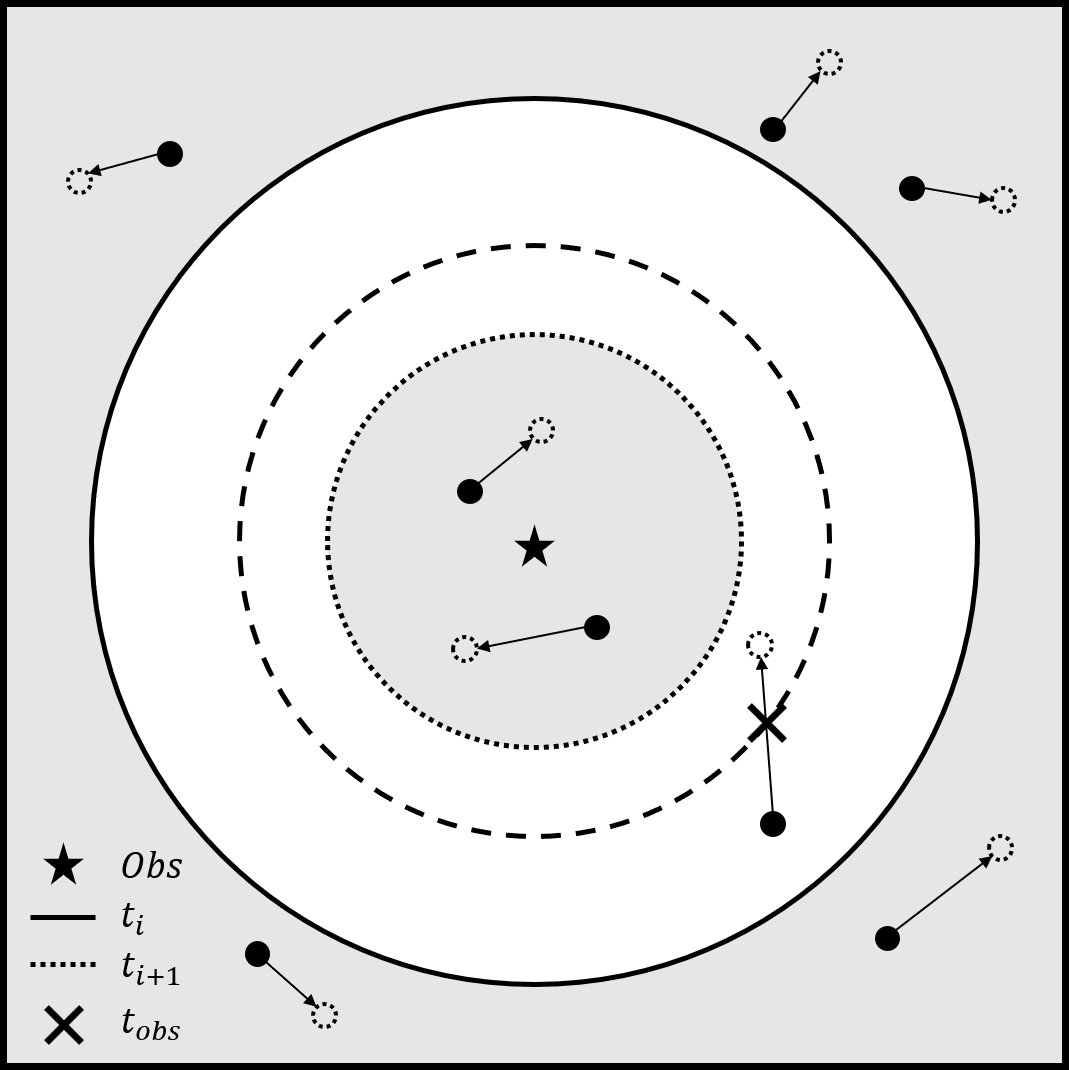
\includegraphics[width=0.5\linewidth]{plots/background/crossing_condition.png}
    \caption{\cite{noauthor_examplepkdgrav3_lightcone_2022}}
    \label{fig:placeholder}
\end{figure}


\subsection{Neural Network}
\subsubsection{Dimensional Reduction}
VRAM issues -> patches or in spherical harmonics
\subsubsection{Data preparation}
\subsubsection{Network Architecture}
\subsubsection{Training Procedure}
\subsubsection{Validation Strategy}
(Angular) Power Spectru, Kappa -> UFALCON 


\section{Computational Infrastructure}
\subsection{Computing Environments}

The code development went through several stages. Starting locally with only testing and seeing how things works towards more complex architecture inside of an cluster. 

\subsubsection{Local Development}

We first implemented disco and pkdgrav on a local device, to see what it needs to run. This also makes sense, since one have direct ouptut, which can be checked and fixed directly. This much more time efficient, than when dealing with clusters. For some simple tests we used a low resolution $res=16$, which lead to a total particle number of $16^3=4096$. A local setup can easily deal with it and also terminate under minute. The problem starts when we want to have higher resolutions, this lead directly to RAM error, since 
\[
res=832 \rightarrow 832^3 = 5\cdot10^8 \text{ particles} \rightarrow ... \text{GB},
\]
which is mostly not available on simple computers. 

\subsubsection{Euler (ETH)}

On the cluster we have created virtual environments for each module (pkdgrav, disco), since some libraries conflict with others and therefore we have to treat it seperately.  But regarding the resources we are now able to use higher resolutions as $res=832$. We can also use GPU supported version, which can lead to a massive speed up. Nevertheless the allocations for this simulations can lead to a rather long runtime depending on what configuration is used. We can therefore adapt to handle multi-node configurations.

\subsubsection{CSCS (Alps/Piz Daint)}

Here we can use the very efficient NVIDIA GH200 with 120 GB of VRAM. This is perfect for scaling up and to reduce the runtimes for each simulation, either for generating the training pairs or for a training of the model itself.  

\subsection{Software Engineering}
\subsubsection{Code Structure}

We saved all the important executable and virtual environments side of the HOME directory of the cluster, since it's not dropped at any times. Since the storage in home is limited to a specific amount, we saved the output into SCRATCH. For example we submitted a transfer job from globus to entrypoint of CSCS to transfer all data from Cosmogridv1 of size 110 $TB$. But also for sure much smaller size of data as for example all logs for each job submission. This was very helpful for debugging and also for later look ups, to compare. Also important plots of snpashots and shells are stored inside of that. 



\subsubsection{ Job Scheduling and Submissions}

For each python script we have also created an bash file. This was very useful since the python script could be used locally, but also on the cluster and the bash file of it was inside of the cluster for job submission either with $sbatch$ or $bash$. That way we were able to control, if we want to monitor output very fast inside of the terminal or if we want to run it in the background and store it. 


\subsubsection{Version Control (GitHub)}

A very important decision was to create a new repository for the project (all scripts) and also the modified DISCO with shell builder. This is useful to have certain safety, if the computer crashes or when losing overview. So there is always the possibility to restore an older working version. 


\section{Results}
from \cite{defferrard_deepsphere_2020}
\section{Conclusion}


\printbibliography

\end{document}


